\documentclass[smaller]{beamer}
\usetheme[english]{Berlin}
%\usepackage{ngerman}
\usepackage[ngerman]{babel}
\useoutertheme{infolines}
\beamertemplatenavigationsymbolsempty
\setbeamertemplate{caption}[numbered]
\usepackage{pgfplots,tikz,subfigure}
\usepackage{amsmath,amsthm}
\usepackage{hyperref,graphics,graphicx,color,algorithm,algorithmic,enumerate}
\usepackage{mymacros,wrapfig,relsize}
\usepackage{pict2e}
\usepackage[utf8x]{inputenc}
\usepackage{csquotes}

\newcommand{\ri}{\mathrm{i}}
\newcommand{\T}{\mathsf{T}}
\renewcommand{\H}{\mathsf{H}}
\newcommand{\eps}{\varepsilon}
\newcommand{\To}{\rightarrow}
\newcommand{\sddots}{\scalebox{0.6}{$\ddots$}}
\usepackage[pdf]{pstricks}
\usepackage{sansmathfonts}
\usepackage{eurosym}
\usepackage{ulem}
%\usepackage{arev}
%\renewcommand\familydefault{\sfdefault}

\DeclareMathOperator{\loc}{loc}
\DeclareMathOperator{\rank}{rank}
\DeclareMathOperator{\RE}{Re}
\DeclareMathOperator{\IM}{Im}
\DeclareMathOperator{\In}{In}
\DeclareMathOperator{\im}{im}
\DeclareMathOperator{\Gl}{Gl}
\DeclareMathOperator{\spa}{span}
\DeclareMathOperator{\ext}{{ext}}
\DeclareMathOperator{\ind}{ind}
\DeclareMathOperator{\normalrank}{normalrank}
\DeclareMathOperator{\essup}{ess\,sup}
\DeclareMathOperator{\vect}{vec}

\newcommand{\re}{\mathrm{e}}
\newcommand{\ddt}{\tfrac{\mathrm{d}}{\mathrm{d}t}}
\newcommand{\sys}[4]{\left[\begin{array}{c|c} #1 & #2 \\ \hline #3 & #4 \end{array}\right]}

\renewcommand{\tilde}{\widetilde}
\renewcommand{\hat}{\widehat}


\title[]{Optimierung f\"ur Studierende der Informatik}
\subtitle{-- 11. Vorlesung --}
\author[Matthias Voigt]{\textbf{Matthias Voigt$^{1,2}$}}
\institute[]{
\begin{columns}
%\begin{center}
\column{0.45\textwidth}{\centering {$^1$Universit\"at Hamburg \\ Fachbereich Mathematik \\ Hamburg \\ }}
\column{0.45\textwidth}{\centering {$^2$Technische Universit\"at Berlin \\ Institut f\"ur Mathematik \\ Berlin  \\}}
%\end{center}
\end{columns}
}
\date[]{Universit\"at Hamburg
\begin{columns}
\column{0.45\textwidth}{\centering \includegraphics[width = 1.2\textwidth]{uhh-logo.png}\\}
\end{columns}
}

\definecolor{tucgreen}{rgb}{0.0,0.5,0.27}
\definecolor{tucred}{rgb}{0.75,0,0}
\definecolor{tucorange}{rgb}{1.0,.5625,0}
\definecolor{mpired}{HTML}{990000}
\definecolor{mpigreen}{HTML}{5C871D}
\definecolor{mpiblue}{HTML}{006AA9}
\definecolor{mpibg1}{HTML}{5D8B8A}
\definecolor{mpibg2}{HTML}{BFDFDE}
\definecolor{mpibg3}{HTML}{A7C1C0}
\definecolor{mpibg4}{HTML}{7DA9A8}
\definecolor{mpigrey}{rgb}{0.9294,0.9294,0.8784}

\begin{document}

\maketitle

\begin{frame}
\frametitle{Kürzeste Pfade in Graphen}
Wir betrachten gerichtete Graphen $G=(V,E)$, in denen jeder Kante $e$ eine reelle Zahl $\ell(e) \geq 0$ zugeordnet ist, die wir die \structure{Länge} von $e$ nennen.

\begin{center}
 \includegraphics{fig74.pdf}
\end{center}

Je nach Anwendung kann man sich unter den Zahlen $\ell(e)$ auch etwas anderes als Längen vorstellen, beispielsweise \alert{Kosten, Zeitangaben oder Wahrscheinlichkeiten.}
\end{frame}

\begin{frame}
\frametitle{Ein grundlegendes algorithmisches Problem}
\textbf{Ein grundlegendes algorithmisches Problem:} Gegeben seien $u,v \in V$. Finde in $G$ einen kürzesten Pfad von $u$ nach $v$ (sofern ein solcher existiert). \\ \vspace*{0.2cm}

Die \structure{Länge $\ell(P)$ eines $u,v$-Pfades $P$} ist dabei wie folgt definiert: Durchläuft $P$ nacheinander die Kanten $e_1,\ldots,e_t$, so gilt
\[
\ell(P) = \sum\limits_{i=1}^t{\ell(e_i)}.
\]

Wir haben unser \enquote{grundlegendes Problem} als ein \enquote{point-to-point} Problem formuliert. In vielen Fällen will man aber mehr wissen: Man fragt nach kürzesten Pfaden von einem festen Knoten $s$ (\enquote{Startpunkt}) \alert{zu allen anderen Knoten} $v$. \\ \vspace*{0.2cm}

Wenn nichts anderes gesagt ist, wollen wir voraussetzen, dass es zu jedem Knoten $v$ des betrachteten Graphen mindestens einen $s,v$-Pfad gibt. Unser Problem lässt sich dann wie folgt formulieren.
\end{frame}

\begin{frame}
\frametitle{Version \enquote{one-to-all}}
Wenn nichts anderes gesagt ist, wollen wir voraussetzen, dass es zu jedem Knoten $v$ des betrachteten Graphen mindestens einen $s,v$-Pfad gibt. Unser Problem lässt sich dann wie folgt formulieren. \\ \vspace*{0.2cm}
\textbf{Problem der kürzesten Pfade (Version: \enquote{one-to-all}):}
Gegeben seien ein gerichteter Graph $G=(V,E)$ mit Kantenlängen $\ell(e) \in \R$, $\ell(e) \geq 0$, sowie ein Knoten $s \in V$. Finde kürzeste Pfade von $s$ zu allen anderen Knoten. 
\end{frame}

\begin{frame}
\frametitle{Ungerichtete Graphen}
Wir haben das Problem der kürzesten Pfade für \alert{gerichtete} Graphen formuliert. Ein entsprechendes Problem für ungerichtete Graphen gesondert zu betrachten, ist nicht nötig, da man den ungerichteten Fall auf den gerichteten zurückführen kann. \\ \vspace*{0.2cm}

\alert{Dies ist durch einen sehr einfachen Trick zu erreichen: Man ersetzt, wie in der folgenden Zeichnung angedeutet, jede ungerichtete Kante durch zwei gerichtete Kanten derselben Länge.}

\begin{center}
\includegraphics{fig75.pdf}
\end{center}
\end{frame}

\begin{frame}
\frametitle{Wichtig: $\ell(e) \ge 0$ für alle Kanten}
Der Algorithmus, den wir im Folgenden besprechen, ist der sehr bekannte \structure{Algorithmus von Dijkstra}, bei dem es sich -- wie wir noch sehen werden -- um einen Greedy-Algorithmus handelt. Wir erwähnen bereits jetzt, dass der Algorithmus nur deshalb korrekt arbeitet, \alert{weil wir $\ell(e) \geq 0$ für alle Kanten $e$ vorausgesetzt haben.} \\ \vspace*{0.2cm}

Der Fall, dass auch Kanten negativer Länge ($\ell(e) < 0$) auftreten, erfordert etwas kompliziertere Methoden -- da kommt man mit einem einfachen Greedy-Verfahren nicht mehr zum Ziel. Wir werden diesen Fall später behandeln.
\end{frame}

\begin{frame}
\frametitle{Die bereits erforschte Menge $S$}
Wir beschreiben den Algorithmus von Dijkstra in einer Variante, bei der \alert{nur die Längen der kürzesten Pfade} ermittelt werden. Es ist jedoch einfach, den Algorithmus so zu ergänzen, dass auch die kürzesten Pfade selbst mitgeliefert werden. \\ \vspace*{0.2cm}

Im Algorithmus von Dijkstra spielt eine Menge $S \subseteq V$ eine wichtige Rolle: Wir nennen $S$ den \alert{bereits erforschten Teil des Graphen}, da in jeder Phase des Algorithmus für die Knoten $u$ der aktuellen Menge $S$ ein Wert $d(u)$ vorliegt, von dem wir nachweisen werden, dass er die Länge eines kürzesten $s,u$-Pfades von $G$ bereits korrekt angibt. \\ \vspace*{0.2cm}

Darüber hinaus gilt sogar, dass es einen solchen Pfad gibt, der ganz in $S$ verläuft.
\end{frame}

\begin{frame}
\frametitle{Von $S = \{s\}$ zu $S=V$}
Am Anfang gilt $S= \bigl\{ s\bigr\}$ und $d(s) = 0$; im Laufe des Algorithmus kommen dann schrittweise Knoten zu $S$ hinzu, bis am Ende $S=V$ gilt. \\ \vspace*{0.2cm}

\textbf{Genauer:} Gilt $S \neq V$, so betrachtet man diejenigen Knoten $v \in V \setminus S$, die von $S$ aus direkt erreichbar sind, d.h., zu denen mindestens eine Kante $e=(u,v)$ mit $u \in S$ führt. Für jeden solchen Knoten $v \in V \setminus S$ stellt man sich vor, \alert{dass die minimale Länge eines $s,v$-Pfades zu berechnen ist, der -- abgesehen von $v$ und seiner letzten Kante $e=(u,v)$ -- ganz in $S$ verläuft} (siehe Zeichnung). 

\begin{center}
 \includegraphics{fig76.pdf}
\end{center}
\end{frame}

\begin{frame}
\frametitle{Der Dijkstra-Algorithmus}
Dementsprechend betrachtet man die Größe
\[
d'(v) = \min{\big\{ d(u) + \ell(u,v) : u \in S \text{ und } (u,v) \in E \big\}}.
\]

In Worten: Für alle $u \in S$, von denen eine Kante $(u,v) \in E$ zu $v$ führt, betrachtet man die Summe $d(u) + \ell(u,v)$; $d'(v)$ ist dann der kleinste unter den betrachteten Werten. \\ \vspace*{0.2cm}

Im Algorithmus von Dijkstra wird nun dasjenige $v \in V \setminus S$ ausgewählt, für das $d'(v)$ so klein wie möglich ist; dieses $v$ wird zu $S$ hinzugefügt und $d(v)$ wird dadurch definiert, dass man $d(v) = d'(v)$ setzt. \\ \vspace*{0.2cm}

Es ergibt sich der folgende Algorithmus:
\end{frame}

\begin{frame}
\frametitle{Der Dijkstra-Algorithmus}
\begin{center}
\label{page:12:1}
\begin{tabular}{rl}
\multicolumn{2}{l}{\textbf{Dijkstra-Algorithmus für $(G, \ell, s)$}} \\
 (1)& Sei $S$ die Menge der bereits erforschten Knoten. \\
 (2)& Für jedes $u \in S$, speichere eine Distanz $d(u)$. \\
 (3)& Am Anfang ist $S = \{ s \}$ und $d(s)=0$. \\
 (4)& \textbf{while} $S \neq V$ \\
 (5)& \qquad Wähle einen Knoten $v \in V \setminus S$ mit mindestens einer Kante von $S$  \\
    & \qquad nach $v$ sodass $d'(v) = \min{\{ d(u) + \ell(u,v) : \ u \in S \text{ and } (u,v) \in E \}}$ \\
    & \qquad so klein wie möglich ist. \\
 (6)& \qquad Füge $v$ zu $S$ hinzu und definiere $d(v) = d'(v)$. \\
 (7)& \textbf{end while}
\end{tabular}
\end{center}

Am Ende liefert der Algorithmus von Dijkstra zu jedem $v \in V$ einen Wert $d(v)$. Noch wissen wir nicht, ob $d(v)$ tatsächlich die Länge eines kürzesten $s,v$-Pfades von $G$ angibt -- das wird erst später nachgewiesen werden. 
\end{frame}

\begin{frame}
\frametitle{Ein Pfad $P_v$ der Länge $d(v)$}
Wir wollen uns zunächst nur davon überzeugen, \alert{dass es überhaupt einen $s,v$-Pfad $P_v$ in $G$ gibt, der die Länge $d(v)$ besitzt.} \\ \vspace*{0.2cm}

Dies ist nicht schwer einzusehen; \alert{man erhält einen solchen Pfad $P_v$ für $v \neq s$ dadurch, dass man im Algorithmus von Dijkstra eine leichte Erweiterung vornimmt:} Bei Aufnahme von $v \neq s$ in die Menge $S$ speichert man zusätzlich immer eine Kante $(u,v)$, die für die Aufnahme von $v$ in $S$ \enquote{verantwortlich} ist, d.h., man speichert eine Kante $(u,v)$ mit $u \in S$, für die $d(u) + \ell(u,v)$ minimal ist. \\ \vspace*{0.2cm}

Um einen $s,v$-Pfad $P_v$ der Länge $d(v)$ für $v \neq s$ zu erhalten, braucht man dann nur noch die entsprechenden Kanten rückwärts zu durchlaufen. \\ \vspace*{0.2cm}

%Man startet in $v$ und durchläuft die für $v$ gespeicherte Kante $(u,v)$ rückwärts; dadurch kommt man von $v$ zum Knoten $u$, der früher als $v$ in $S$ aufgenommen wurde. Falls $u \neq s$, so durchläuft man danach die zu $u$ gespeicherte Kante $(w,u)$ rückwärts und kommt zum Knoten $w$, der noch früher in $S$ aufgenommen wurde. Dies führt man fort, bis man bei $s$ angelangt ist. Durchläuft man diese Kanten umgekehrt von $s$ nach $v$, so erhält man den gewünschten $s,v$-Pfad $P_v$ der Länge $d(v)$.

Man definiert zusätzlich den Pfad $P_s$ als den nur aus $s$ bestehenden Pfad der Länge 0.
\end{frame}

\begin{frame}
\frametitle{Ein Pfad $P_v$ der Länge $d(v)$}

Zu jedem vom Algorithmus gelieferten Wert $d(v)$ gehört also ein $s,v$-Pfad $P_v$, der die Länge $d(v)$ besitzt und den man wie beschrieben erhält. Weiter unten werden wir uns davon überzeugen, dass dieser $s,v$-Pfad $P_v$ sogar immer ein \alert{kürzester $s,v$-Pfad von $G$} ist. Wir halten dieses Ergebnis bereits hier fest:
\begin{equation}
\label{eq:12:2}
\begin{array}{c}
\alert{\text{Der vom Algorithmus von Dijkstra gelieferte Wert $d(v)$ gibt für jeden }} \\
\alert{\text{Knoten $v$ die Länge eines kürzesten $s,v$-Pfades in $G$ an und der}} \\
\alert{\text{dazugehörige Pfad $P_v$ ist ein solcher kürzester Pfad.}}
\end{array}
\end{equation}

Wir schauen uns den Ablauf des Algorithmus von Dijkstra anhand eines \textbf{Beispiels} an; $G$ sei der folgende Graph:
\end{frame}

\begin{frame}
\frametitle{Ein Beispiel}
\begin{center}
 \includegraphics{fig77.pdf}
\end{center}
\end{frame}

\begin{frame}
\frametitle{Ablauf des Algorithmus}
\textbf{Initialisierung:}

Es sei $S = \bigl\{ s \bigr\}$ und $d(s) = 0$. \\ \vspace*{0.2cm}

\textbf{1.	Durchlauf der While-Schleife:} 

Die Knoten aus $V \setminus S$, zu denen Kanten aus $S$ führen, sind $u$, $v$, $x$; man erhält $d'(u) = 1$, $d'(v) = 2$, $d'(x) = 4$. Es folgt $S = \bigl\{ s,u \bigr\}$ und $d(u) = 1$. \\ \vspace*{0.2cm}

\textbf{2.	Durchlauf der While-Schleife:} 

Die Knoten aus $V \setminus S$, zu denen Kanten aus $S$ führen, sind $v$, $x$, $y$; man erhält $d'(v) = 2$, $d'(x) = 2$, $d'(y) = 4$. Man kann $v$ oder $x$ in $S$ aufnehmen; wir entscheiden uns (willkürlich) für $v$. Es folgt $S = \bigl\{ s,u,v \bigr\}$ und $d(v) = 2$.


\end{frame}

\begin{frame}
\frametitle{Ablauf des Algorithmus}
\textbf{3.	Durchlauf der While-Schleife:} 

Die Knoten aus $V \setminus S$, zu denen Kanten aus $S$ führen, sind $x$, $y$, $z$;  man erhält $d'(x) = 2$, $d'(y) = 4$, $d'(z) = 5$. Es folgt $S = \bigl\{ s,u,v,x \bigr\}$ und $d(x) = 2$. \\ \vspace*{0.2cm}


\textbf{4.	Durchlauf der While-Schleife:} 

Die Knoten aus $V \setminus S$, zu denen Kanten aus $S$ führen, sind $y$ und $z$;  man erhält $d'(y) = 3$, $d'(z) = 4$. Es folgt $S = \bigl\{ s,u,v,x,y \bigr\}$ und $d(y) = 3$. \\ \vspace*{0.2cm}

\textbf{5.	Durchlauf der While-Schleife:} 

Für den verbliebenen Knoten $z$ erhält man $d'(z)=4$. Es folgt $S = \bigl\{ s,u,v,x,y,z \bigr\}$ und $d(z) = 4$.
\end{frame}

\begin{frame}
\frametitle{Kurzsichtige Vorgehensweise des Dijkstra-Algorithmus}
Der Algorithmus von Dijkstra ist ein Greedy-Algorithmus, da er in jedem Schritt \alert{kurzsichtig} vorgeht: \\ \vspace*{0.2cm}
 
Wenn es darum geht, $S$ zu erweitern, so schaut sich der Algorithmus nur Kanten an, die direkt von $S$ ausgehen -- gerade so, als ob er Kanten, die weiter von $S$ entfernt sind, nicht erkennen könnte. \\ \vspace*{0.2cm}

Bei so viel Kurzsichtigkeit braucht man sich nicht zu wundern, dass der Algorithmus im Allgemeinen keine korrekten Ergebnisse liefert, wenn Kanten negativer Länge im Spiel sind. Hier ein \textbf{Beispiel}, an dem zu erkennen ist, was im Falle negativer Kantenlängen schiefgehen kann:
\end{frame}

\begin{frame}
\frametitle{Ein Beispiel mit negativen Kantenlängen}
\begin{center}
\includegraphics{fig78.pdf}
\end{center}
Wenden Sie den Algorithmus von Dijkstra auf diesen Beispielgraphen an und finden Sie heraus, \alert{was schief geht!}
\end{frame}

\begin{frame}
\frametitle{Der Dijkstra-Algorithmus: Korrektheitsbeweis}
Wir setzen nun wieder $\ell(e) \geq 0$ für alle Kanten $e$ voraus und kommen zum Beweis von \eqref{eq:12:2} (\enquote{Korrektheitsbeweis für den Algorithmus von Dijkstra}). Da der Algorithmus von Dijkstra der vielleicht bekannteste Algorithmus zum Berechnen von kürzesten Pfaden in Graphen ist, findet man Beweise für seine Korrektheit in vielen Lehrbüchern. Wir schauen uns die \alert{Darstellung von Kleinberg und Tardos an:} \\ \vspace*{0.2cm}

Wir zeigen gleich:
\begin{equation}
\label{4.14}
\begin{array}{c}
\alert{\text{Betrachte die Menge $S$ an einem beliebigen Punkt während der Ausführung}}\\
\alert{\text{des Algorithmus. Für jedes $u \in S$ ist der Pfad $P_u$ ein kürzester $s,u$- Pfad.}}
\end{array}
\end{equation}
Dieser Fakt beweist direkt die Korrektheit des Dijkstra-Algorithmus, denn wir können ihn anwenden, sobald der Algorithmus terminiert und $S$ somit alle Knoten enthält. 

\end{frame}

\begin{frame}
\frametitle{Der Dijkstra-Algorithmus: Korrektheitsbeweis}
\textbf{Beweis von \eqref{4.14}:} Wir beweisen die Aussage per Induktion über die Größe von $S$. Der Fall $|S| = 1$ ist einfach, da wir dann $S = \big\{ s \big\}$ und $d(s) = 0$ haben. Angenommen die Behauptung gilt für $|S| = k$ und ein $k \geq 1$; wir vergrößern $S$ auf Größe $k + 1$ durch Hinzufügen des Knotens $v$. Sei $(u, v)$ die letzte Kante im $s,v$-Pfad $P_v$. \\ \vspace*{0.2cm}

Wegen der Induktionsannahme ist $P_u$ der kürzeste $s,u$-Pfad für jedes $u \in S$. Betrachte nun einen beliebigen anderen $s,v$-Pfad $P$; wir wollen zeigen, dass dieser mindestens so lang ist wie $P_v$. Um $v$ zu erreichen muss dieser Pfad $P$ die Menge $S$ \alert{irgendwo} verlassen; sei $y$ der erste Knoten in $P$, der nicht in $S$ liegt und sei $x \in S$ der Knoten, der genau vor $y$ kommt.
\end{frame}

\begin{frame}
\frametitle{Der Dijkstra-Algorithmus: Korrektheitsbeweis}
\begin{center}
 \includegraphics[scale = 0.8]{fig79.pdf}
\end{center}

Die Situation ist in der Abbildung illustriert und die \alert{Idee des Beweises} ist sehr einfach: $P$ kann nicht kürzer als $P_v$ sein da es bereits mindestens so lang wie $P_v$ zum Zeitpunkt des Verlassens von $S$ ist. Tatsächlich muss der Dijkstra-Algorithmus in Iteration $k + 1$ das Hinzufügen von $y$ zur Menge $S$ über die Kante $(x, y)$ betrachten -- aber diese Möglichkeit verworfen haben, um $v$ hinzuzufügen. 
\end{frame}

\begin{frame}
\frametitle{Der Dijkstra-Algorithmus: Korrektheitsbeweis}
Das bedeutet dass kein Pfad von $s$ nach $y$ durch $x$ existiert, der kürzer ist als $P_v$. Aber der Teilpfad von $P$ bis nach $y$ ist ein solcher Pfad und somit ist dieser Teilpfad mindestens so lang wie $P_v$. Da alle Kantenlängen nichtnegativ sind, muss der ganze Pfad $P$ auch mindestens so lang sein wie $P_v$. \qquad $\Box$ \\ \vspace*{0.2cm}
Der obige Beweis der Korrektheit des Algorithmus von Dijkstra läuft übrigens nach dem Schema \alert{\enquote{the greedy algorithm stays ahead}} ab: Der Algorithmus von Dijkstra baut die Gesamtlösung schrittweise auf und im Beweis wird gezeigt, dass die vom Dijkstra-Algorithmus in diesem Prozess gelieferten Teillösungen für die Mengen $S$ bereits optimal sind (und deshalb von keinem anderen Algorithmus übertroffen werden können). \\ \vspace*{0.2cm}

\textbf{Anders gesagt:} Es wird gezeigt, dass der Dijkstra-Algorithmus für jede Menge $S$ \alert{\enquote{vorne liegt}.}

\end{frame}

\begin{frame}
\frametitle{Wie ermittelt man den Knoten $v$ auf effiziente Art?}
Ein \alert{wichtiges Detail} fehlt noch: \alert{Die Frage, wie man in jedem Durchlauf der While-Schleife den Knoten $v$ auf eine effiziente Art findet, wurde bislang ausgespart.} \\ \vspace*{0.2cm}

Auf den ersten Blick hat man den Eindruck, dass man wie folgt vorgehen müsste: Für jeden Knoten $v \notin S$, zu dem mindestens eine von $S$ ausgehende Kante hinführt, hat man für sämtliche Kanten $e = (u,v)$ mit $u \in S$ den Wert $d(u) + \ell(e)$ zu bilden und $v$ das Minimum $d'(v)$ all dieser Werte zuzuordnen. \\ \vspace*{0.2cm}

Unter allen $v \notin S$, denen auf diese Art ein $d'(v)$ zugeordnet wurde, wählt man sich dann einen Knoten $v$, für den $d'(v)$ so klein wie möglich ist. Dieses $v$ nimmt man zu $S$ hinzu, setzt $d(v) = d'(v)$ und steigt ggf. in den nächsten Durchlauf der While-Schleife ein.
\end{frame}

\begin{frame}
\frametitle{Wie ermittelt man den Knoten $v$ auf effiziente Art?}
Im nächsten Durchlauf der While-Schleife könnte man nun ganz entsprechend vorgehen; dabei würde man jedoch merken, dass etliche Rechnungen, die bereits im vorangegangenen Durchlauf der While-Schleife durchgeführt wurden, nur wiederholt werden. In manchen Fällen würden sich die im vorangegangenen Durchlauf berechneten Werte \alert{nicht ändern:}
\begin{itemize}
\item Wurde beim vorangegangenen Durchlauf der While-Schleife $v$ zu $S$ hinzugefügt und ist für einen Knoten $w \notin S$ die Kante $(v,w)$ nicht vorhanden, so ändert sich der Wert $d'(w)$ gegenüber dem vorangegangenen Durchlauf nicht, da es immer noch genau dieselben Kanten $e=(u,w)$ sind, die zur Berechnung von $d'(w)$ herangezogen werden.

\item \alert{Und wie ändert sich der Wert $d'(w)$ für ein $w \notin S$, wenn die Kante $(v,w)$ vorhanden ist?} Offenbar hat man den alten Wert $d'(w)$ mit dem Wert $d(v) + \ell(v,w)$ zu vergleichen und hierbei nach der folgenden Update-Formel vorzugehen:
\[
d'(w) = \min{\big\{ d'(w), d(v)+\ell(v,w) \big\}}.
\]
\end{itemize}
\end{frame}

\begin{frame}
\frametitle{Modifizierte Version des Dijkstra-Algorithmus}
Es wäre also unökonomisch, die erhaltenen Werte $d'(w)$ am Ende des vorangegangenen Durchlaufs der While-Schleife einfach \enquote{wegzuschmeißen}. Diese Überlegungen führen zur folgenden \structure{modifizierten Version des Algorithmus von Dijkstra.}

\begin{center}
\label{page:12:2}
\begin{tabular}{rl}
\multicolumn{2}{l}{\textbf{modifizierter Dijkstra-Algorithmus für $(G, \ell, s)$}} \\
 (1)& Sei $S$ die Menge der bereits erforschten Knoten. \\
 (2)& Für jedes $u \in S$, speichere eine Distanz $d(u)$. \\
 (3)& Am Anfang ist $S = \{ s \}$ und $d(s)=0$. \\
 (4)& Für jedes $u \neq s$ sei $d(u) = \ell(s,u)$, falls $(s,u)\in E$ \\
    & und andernfalls $d(u)=\infty$. \\
 (5)& \textbf{while} $S \neq V$. \\
 (6)& \qquad Wähle einen Knoten $v \in V \setminus S$ mit $d(v) = \min{\big\{ d(u) : u \in V \setminus S \big\}}$. \\
 (7)& \qquad Füge $v$ zu $S$ hinzu. \\
 (8)& \qquad Für jedes $u \in V \setminus S$ mit $(v,u) \in E$ setze \\
    & \qquad $d(u) = \min{\bigl\{ d(u), d(v) + \ell(v,u) \bigr\}}$. \\
 (9)& \textbf{end while}
\end{tabular}
\end{center}
\end{frame}

\begin{frame}
\frametitle{Laufzeit}
Die Laufzeit dieser Version des Dijkstra-Algorithmus ist \alert{$O(n^2)$} für $n = |V|$, da die While-Schleife $n-1$ mal durchlaufen wird und die Zeilen (6)--(8) offenbar in $O(n)$ Zeit ausgeführt werden können. \\ \vspace*{0.2cm}

Liegt ein dichtbesetzter Graph vor, d.h., für $m=|E|$ gilt $m = \Theta(n^2)$, so ist die Laufzeitschranke $O(n^2)$ bestmöglich, da jede Kante inspiziert werden muss. \\ \vspace*{0.2cm}

Ist $m$ dagegen asymptotisch kleiner als $n^2$, so lassen sich durch Einsatz geeigneter Datenstrukturen Laufzeitverbesserungen erreichen (vgl. etwa Kleinberg/Tardos).
\end{frame}

\begin{frame}
\frametitle{Vorläufige und endgültige Werte $d(u)$}
Bevor wir die Arbeitsweise des Algorithmus anhand eines Beispiels illustrieren, noch ein Wort zu den Werten $d(u)$: 
\begin{itemize}
\item Für $u \in S$ gibt $d(u)$ wie bisher die Länge eines kürzesten $s,u$-Pfades in $G$ an. 
\item Für Knoten $u \notin S$, zu denen mindestens eine von $S$ ausgehende Kante hinführt, bezeichnet $d(u)$ die Größe, die wir bislang $d'(u)$ genannt haben;
\item für die übrigen Knoten $u \notin S$ gilt $d(u) = \infty$.
\end{itemize}  \vspace*{0.2cm}
Für alle $u \in V \setminus S$ gibt $d(u)$ somit eine \alert{obere Schranke} für die Länge eines kürzesten $s,u$-Pfades in $G$ an; der Wert $d(u)$ kann in diesem Fall noch verändert werden; er ist \alert{vorläufig}. Nach Aufnahme von $u$ in $S$ ändert sich der Wert von $d(u)$ nicht mehr -- er ist \alert{endgültig} und gibt den Abstand von $s$ und $u$ in $G$ an.
\end{frame}

\begin{frame}
\frametitle{Ein Beispiel zum Dijkstra-Algorithmus}
 \textbf{Beispiel:} Der Graph $G=(V,E)$ mit Längenfunktion $\ell$ sei durch die folgende Zeichnung gegeben:

\begin{center}
 \includegraphics{fig80.pdf}
\end{center}

Wir geben für jeden Knoten $u$ an, welchen Wert $d(u)$ nach der Initialisierung und nach jedem Durchlauf der While-Schleife besitzt. Außerdem wird das jeweils aktuelle $S$ angegeben. Ist ein Wert $d(u)$ endgültig (man sagt auch \alert{permanent}), so wird er unterstrichen.
\end{frame}

\begin{frame}
\frametitle{Ein Beispiel zum Dijkstra-Algorithmus}
\textbf{Initialisierung:}
\[
S = \big\{ s \big\}
\]
\begin{center}
\begin{tabular}{c|ccccc}
$u$ & $s$ & $a$ & $b$ & $c$ & $e$ \\ \hline
$d(u)$ & $\underline{0}$ & 4 & 2 & $\infty$ & $\infty$
\end{tabular}
\end{center}

\textbf{1. Durchlauf der Schleife:}
\[
S = \big\{ s,b \big\}
\]
\begin{center}
\begin{tabular}{c|ccccc}
$u$ & $s$ & $a$ & $b$ & $c$ & $e$ \\ \hline
$d(u)$ & $\underline{0}$ & $3$ & $\underline{2}$ & $6$ & $7$
\end{tabular}
\end{center}

\textbf{2. Durchlauf der Schleife:}
\[
S = \big\{ s,b,a \big\}
\]
\begin{center}
\begin{tabular}{c|ccccc}
$u$ & $s$ & $a$ & $b$ & $c$ & $e$ \\ \hline
$d(u)$ & $\underline{0}$ & $\underline{3}$ & $\underline{2}$ & $5$ & $6$
\end{tabular}
\end{center}
\end{frame}

\begin{frame}
\frametitle{Ein Beispiel zum Dijkstra-Algorithmus}
\textbf{3. Durchlauf der Schleife:}
\[
S = \big\{ s,b,a,c \big\}
\]
\begin{center}
\begin{tabular}{c|ccccc}
$u$ & $s$ & $a$ & $b$ & $c$ & $e$ \\ \hline
$d(u)$ & $\underline{0}$ & $\underline{3}$ & $\underline{2}$ & $\underline{5}$ & $6$
\end{tabular}
\end{center}

\textbf{4. Durchlauf der Schleife:}
\[
S = \big\{ s,b,a,c,e \big\}
\]
\begin{center}
\begin{tabular}{c|ccccc}
$u$ & $s$ & $a$ & $b$ & $c$ & $e$ \\ \hline
$d(u)$ & $\underline{0}$ & $\underline{3}$ & $\underline{2}$ & $\underline{5}$ & $\underline{6}$
\end{tabular}
\end{center}
\end{frame}

\begin{frame}
\frametitle{Ein Beispiel zum Dijkstra-Algorithmus}
\textbf{Übersichtliche Zusammenfassung:}
\begin{center}
\begin{tabular}{c||c|c|c|c|c||l}
 & $s$ & $a$ & $b$ & $c$ & $e$ & \ $S$ \\ \hline\hline
$0$ & $\underline{0}$ & $4$ & $2$ & $\infty$ & $\infty$ & $\bigl\{ s \bigr\}$ \\ \hline
$1$ & $\underline{0}$ & $3$ & $\underline{2}$ & $6$ & $7$ & $\bigl\{ s,b \bigr\}$ \\ \hline
$2$ & $\underline{0}$ & $\underline{3}$ & $\underline{2}$ & $5$ & $6$ & $\bigl\{ s,b,a \bigr\}$ \\ \hline
$3$ & $\underline{0}$ & $\underline{3}$ & $\underline{2}$ & $\underline{5}$ & $6$ & $\bigl\{ s,b,a,c \bigr\}$ \\ \hline
$4$ & $\underline{0}$ & $\underline{3}$ & $\underline{2}$ & $\underline{5}$ & $\underline{6}$ & $\bigl\{ s,b,a,c,e \bigr\}$
\end{tabular}
\end{center}

Einen kürzeste-Pfade-Baum $\widetilde{B}$ kann man leicht am Graphen ablesen:

\begin{center}
 \includegraphics{fig81.pdf}
\end{center}
\end{frame}

\begin{frame}
\frametitle{Kürzeste-Pfade-Bäume}
 \textbf{Eine Bemerkung zur Terminologie:} Unter einem \structure{Baum} versteht man bekanntlich einen ungerichteten Graphen, der kreislos und zusammenhängend ist. Im Sinne dieser Definition ist der \enquote{kürzeste-Pfade-Baum} $\widetilde{B}$ (streng genommen) gar kein Baum, da $\widetilde{B}$ ein gerichteter Graph ist. Die Bezeichnung von $\widetilde{B}$ als \enquote{kürzester-Pfade-Baum} ist trotzdem üblich: \\ \vspace*{0.2cm}
 
 \alert{Das rechtfertigt sich dadurch, dass es einen Baum $B$ mit Wurzel $s$ gibt, von dem $\widetilde{B}$ \enquote{abstammt}. Das soll heißen: $\widetilde{B}$ entsteht aus $B$ dadurch, dass man alle Kanten von $s$ weg orientiert.}
\end{frame}

\begin{frame}
\frametitle{Systematische Vorgehensweise}
\alert{Um einen kürzeste-Pfade-Baum \textit{systematisch} zu finden, ist der Algorithmus von Dijkstra zu erweitern:} Für $u \neq s$ speichert man im Fall $d(u) \neq \infty$ nicht nur den Wert $d(u)$, sondern auch einen dazugehörigen \enquote{Vorgängerknoten} $w$ aus $S$, d.h., nach dem $i$-ten Durchlauf der While-Schleife gilt $d(u) = d(w) + \ell(w,u)$ für den angegebenen Knoten $w \in S$. \\ \vspace*{0.2cm}

\textbf{Im Beispiel sieht das so aus:}

\begin{center}
\begin{tabular}{c||c|c|c|c|c||l}
 & $s$ & $a$ & $b$ & $c$ & $e$ & \ $S$ \\ \hline\hline
$0$ & $\underline{0}$ & $4\ s$ & $2\ s$ & $\infty$ & $\infty$ & $\bigl\{ s \bigr\}$ \\ \hline
$1$ & $\underline{0}$ & $3\ b$ & $\underline{2}\ s$ & $6\ b$ & $7\ b$ & $\bigl\{ s,b \bigr\}$ \\ \hline
$2$ & $\underline{0}$ & $\underline{3}\ b$ & $\underline{2}\ s$ & $5\ a$ & $6\ a$ & $\bigl\{ s,b,a \bigr\}$ \\ \hline
$3$ & $\underline{0}$ & $\underline{3}\ b$ & $\underline{2}\ s$ & $\underline{5}\ a$ & $6\ a$ & $\bigl\{ s,b,a,c \bigr\}$ \\ \hline
$4$ & $\underline{0}$ & $\underline{3}\ b$ & $\underline{2}\ s$ & $\underline{5}\ a$ & $\underline{6}\ a$ & $\bigl\{ s,b,a,c,e \bigr\}$
\end{tabular}
\end{center}

Anhand der letzten Zeile kann man zu jedem $u \neq s$ einen Vorgänger auf einem kürzesten $s,u$-Pfad ablesen.
\end{frame}

\begin{frame}
\frametitle{Einrichtung eines Kommunikationsnetzwerkes}
Wir befassen uns in diesem Abschnitt mit einem Problem, das ebenso grundlegend wie das zuvor behandelte Problem der kürzesten Pfade ist. \\ \vspace*{0.2cm}

Gegeben sei eine Menge $V$ von $n$ Knoten, sagen wir $V = \bigl\{ v_1, \ldots, v_n \bigr\}$. Wir stellen uns vor, dass zwischen diesen Knoten ein \alert{Kommunikationsnetzwerk} eingerichtet werden soll. Dabei muss es nicht unbedingt für alle Paare $v_i,v_j$ möglich sein, eine direkte Verbindung einzurichten -- für gewisse Paare $v_i,v_j$ von verschiedenen Knoten soll dies aber infrage kommen, wobei der Aufbau einer solchen direkten Verbindung \alert{Kosten} verursacht. \\ \vspace*{0.2cm}

Kommunikationsverbindungen sollen immer in beide Richtungen nutzbar sein, d.h., zur Modellierung werden wir \alert{ungerichtete Graphen} verwenden. \\ \vspace*{0.2cm}

Das zu errichtende Kommunikationsnetzwerk soll natürlich \alert{zusammenhängend} sein, d.h., zwischen zwei verschiedenen Knoten $v_i$ und $v_j$ soll es immer einen Pfad geben, der $v_i$ mit $v_j$ verbindet. \alert{Das Ziel ist, die Gesamtkosten zu minimieren}.
\end{frame}

\begin{frame}
\frametitle{Das Problem}
Wir gelangen zu folgendem \textbf{Problem:} \\ \vspace*{0.2cm}

\textbf{Gegeben:} ein zusammenhängender Graph $G=(V,E)$; jeder Kante $e \in E$ sei eine reelle Zahl $c(e) > 0$ zugeordnet (\enquote{Kosten von $e$}). \\ \vspace*{0.2cm}

\textbf{Gesucht:} eine Teilmenge $F$ der Kantenmenge $E$, so dass der Graph $(V,F)$ zusammenhängend ist und außerdem die Gesamtkosten
\[
\sum\limits_{e \in F}{c(e)}
\]
minimal sind.
\end{frame}

\begin{frame}
\frametitle{Eine Feststellung über Bäume}
Wir erinnern noch einmal an die Definition eines Baums. \\ \vspace*{0.2cm}

\textbf{Definition:} Unter einem \structure{Baum} versteht man einen ungerichteten Graphen, der zusammenhängend und kreislos ist. \\ \vspace*{0.2cm}

Wir schließen eine \alert{einfache Beobachtung} an. \\ \vspace*{0.2cm}

\textbf{Feststellung:}
\begin{equation}
\label{eq:12:**}
\tag{$\star\star$}
\begin{array}{c}
\alert{\text{Es sei $(V,F)$ eine Lösung unseres Problems, d.h., der Graph $(V,F)$}} \\
\alert{\text{ist zusammenhängend und die Gesamtkosten $\sum\limits_{e \in F}{c(e)}$ sind minimal.}} \\
\alert{\text{Dann ist $(V,F)$ ein Baum.}}
\end{array}
\end{equation}
\end{frame}

\begin{frame}
\frametitle{Minimale aufspannende Bäume}
Ist $G=(V,E)$ ein Graph und $T=(V,F)$ ein Baum mit $F \subseteq E$, so nennt man $T$ einen \structure{aufspannenden Baum} von $G$. \\ \vspace*{0.2cm}

\textbf{Anders gesagt:} Ein aufspannender Baum von $G$ ist ein Teilgraph von $G$, der alle Knoten von $G$ enthält und bei dem es sich um einen Baum handelt. \\ \vspace*{0.2cm}

Die Feststellung \eqref{eq:12:**} besagt, dass als Lösung unseres Problems nur aufspannende Bäume infrage kommen. Gesucht ist also ein \structure{minimaler aufspannender Baum} von $G$ (engl. \structure{minimum spanning tree}, kurz: \structure{MST}).
\end{frame}

\begin{frame}
\frametitle{Ein Satz von Cayley}
Ein Graph $G$ hat -- wenn man einmal von sehr einfachen Fällen absieht -- in der Regel \alert{sehr viele aufspannende Bäume.} \\ \vspace*{0.2cm}

Beispielsweise besagt ein bekannter Satz von Cayley, dass ein vollständiger Graph mit $n$ Knoten genau
\[
n^{n-2}
\]
aufspannende Bäume besitzt. \\ \vspace*{0.2cm}

Es ist also auf den ersten Blick alles andere als klar, wie man unter all diesen Bäumen einen Baum $T=(V,F)$ finden soll, für den 
\[
\sum\limits_{e \in F}{c(e)}
\]
minimal ist.
\end{frame}

\begin{frame}
 \frametitle{Greed works!}
In früheren Beispielen aus dem Gebiet des Schedulings haben wir gesehen, wie leicht es ist, \alert{sich eine Reihe von natürlich erscheinenden Greedy-Algorithmen auszudenken, für die es in jedem Einzelfall durchaus einleuchtende Plausibilitätsargumente gibt.} Häufig funktionierten diese Algorithmen jedoch nicht. \\ \vspace*{0.2cm}

Auch beim Problem des minimalen aufspannenden Baums ist es möglich, sich etliche Greedy-Algorithmen einfallen zu lassen -- \alert{diesmal ist es aber erstaunlicherweise so, dass viele der Greedy-Algorithmen, die einem in den Sinn kommen, auch tatsächlich funktionieren.} Für das Problem des minimalen aufspannenden Baums kann demnach völlig zu Recht behauptet werden: 
\begin{equation*}
\alert{\text{\enquote{Greed works.}}}
\end{equation*}
Hier sind \alert{drei einfache Greedy-Algorithmen} für das Problem des minimalen aufspannenden Baums, die alle drei korrekt arbeiten, d.h., einen minimalen aufspannenden Baum auch tatsächlich finden. Wir beschreiben zunächst diese Algorithmen und kümmern uns erst danach um die Frage nach ihrer Korrektheit.
\end{frame}

\begin{frame}
\frametitle{Kruskals Algorithmus}
Der erste dieser drei Greedy-Algorithmen geht wie folgt vor. Zunächst werden die Kanten von $E$ nach ihren Kosten sortiert, und zwar in aufsteigender Reihenfolge: $e_1,\ldots,e_m$ mit $c(e_i) \leq c(e_{i+1})$ ($i = 1,\ldots,m-1$). \\ \vspace*{0.2cm}

Man startet nun mit dem kantenlosen Graphen $(V, \emptyset)$, geht die aufsteigend sortierten Kanten von links nach rechts durch und stellt jedes Mal die Frage:
\alert{Entsteht ein Kreis, wenn $e_i$ zum bereits konstruierten Teilgraphen hinzugenommen wird?} Falls ja, so wird $e_i$ zurückgewiesen; falls nein, so wird $e_i$ zum bereits konstruierten Teilgraphen hinzugefügt. \\ \vspace*{0.2cm}

Diese Vorgehensweise wird \structure{Kruskals Algorithmus} genannt.
\end{frame}

\begin{frame}
\frametitle{Prims Algorithmus}
Ein anderer, ebenso einfacher Algorithmus weist große Ähnlichkeit mit Dijkstras Algorithmus zum Auffinden kürzester Pfade auf. \\ \vspace*{0.2cm}

Man startet mit einem einzelnen Knoten $s$ (\enquote{Startknoten}, \enquote{Wurzel}) und baut ausgehend von $s$ einen Baum auf, indem man in jedem Schritt eine weitere Kante $e=\big\{u,v\big\}$ hinzunimmt, die genau einen Knoten mit dem bereits konstruierten Teilbaum gemeinsam hat; dabei wird $e$ jedes Mal so gewählt, dass $c(e)$ möglichst klein ist. \\ \vspace*{0.2cm}

Dieses Verfahren wird \structure{Prims Algorithmus} genannt.
\end{frame}

\begin{frame}
\frametitle{Reverse-Delete-Algorithmus}
Der dritte diese Algorithmen kann als eine \enquote{Rückwärtsversion} von Kruskals Algorithmus angesehen werden. \\ \vspace*{0.2cm}

Zunächst werden die Kanten von $E$ wieder nach ihren Kosten sortiert, diesmal aber in absteigender Reihenfolge: $e_1,\ldots, e_m$ mit $c(e_i) \geq c(e_{i+1})$ ($i=1,\ldots,m-1$). Man startet mit dem Graphen $G=(V,E)$, geht die Kanten in der Reihenfolge $e_1,\ldots,e_m$ durch und stellt jedes Mal die Frage: \alert{Bleibt der aktuelle Teilgraph zusammenhängend, wenn man die Kante $e_i$ entfernt?} Falls ja, so wird $e_i$ aus dem aktuellen Teilgraphen entfernt; falls nein, so bleibt $e_i$ im aktuellen Teilgraphen. \\ \vspace*{0.2cm}

Diese Methode wird \structure{Reverse-Delete-Algorithmus} genannt.
\end{frame}

\begin{frame}
\frametitle{Austauschargument}
Woran liegt es nun, dass alle drei beschriebenen Algorithmen korrekt arbeiten, d.h. einen minimalen aufspannenden Baum liefern? Die Antwort, die sich aufgrund der nachfolgenden Analyse ergeben wird, ist, dass ein \alert{Austauschargument}  dahinter steckt. \\ \vspace*{0.2cm}

\textbf{Genauer:} Um die Korrektheit der Algorithmen nachzuweisen, werden wir zunächst einen Hilfssatz vorstellen, der für unsere Zwecke sehr nützlich sein wird. Schaut man sich den Beweisteil d) $\Rightarrow$ a) dieses Hilfssatzes an, so erkennt man: Hier geht es um ein \alert{Austauschargument.} 
\end{frame}

\begin{frame}
\frametitle{Analyse der Algorithmen}
 Alle drei Algorithmen arbeiten ähnlich, nämlich mit wiederholtem Hinzu- bzw. Wegnehmen von Kanten. Um diese Vorgehensweise zu analysieren fragen wir:
\begin{itemize}
\item Kann man beim Algorithmus von Kruskal bzw. Prim sicher sein, dass man nichts falsch macht, wenn man eine Kante zu einer bereits existierenden Teillösung hinzunimmt?
\item Kann man beim Reverse-Delete-Algorithmus sicher sein, dass man keine Kante vorschnell aussortiert hat?
\end{itemize}

Die Antworten auf die aufgeworfenen Fragen werden sich aus dem Folgenden ergeben, wobei wir den Schwerpunkt auf die Analyse der \alert{Algorithmen von Kruskal und Prim} legen.
\end{frame}

\begin{frame}
\frametitle{Das Problem}
Das Problem, um das es geht, lässt sich wie folgt beschreiben:

\medskip
\begin{center}
	\begin{minipage}{0.875\textwidth}
		\textbf{Minimum-Spanning-Tree-Problem}
		
		\medskip
		\textbf{Instanz}: Ein ungerichteter, zusammenhängender Graph $G$ mit Kantengewichten $c(e) > 0$.
		
		\medskip
		\textbf{Aufgabe}: Bestimme einen aufspannenden Baum von $G$ mit minimalem Gewicht.
	\end{minipage}
\end{center}
\end{frame}

\begin{frame}
\frametitle{Einige Bezeichnungen}
Wir beginnen mit der \alert{Zusammenstellung einiger Bezeichnungen}. \\ \vspace*{0.2cm}

Ist ein Graph $G$ gegeben, so bezeichnen wir die Knotenmenge von $G$ mit $V(G)$; $E(G)$ bezeichnet die Kantenmenge von $G$. Für $X \subseteq V(G)$ sei mit $\delta(X)$ die Menge derjenigen Kanten $e \in E(G)$ bezeichnet, für die gilt: Genau ein Endpunkt von $e$ liegt in $X$ (siehe Zeichnung).

\begin{center}
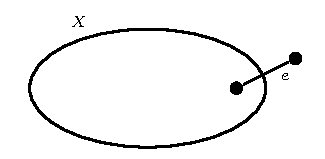
\includegraphics{fig82.pdf}
\end{center}

Man kann die Menge $\delta(X)$ auch so beschreiben:
\[
\delta(X) = \Bigl\{ e \in E(G) : |e \cap X| = 1 \Bigr\}.
\]

\end{frame}

\begin{frame}
\frametitle{Bezeichnungen}
Soll betont werden, dass wir uns auf den Graphen $G$ beziehen, so schreiben wir $\delta_G(X)$ anstelle von $\delta(X)$. \\ \vspace*{0.2cm}

Für $e \in E(G)$ bezeichnet $G-e$ den Graphen, den man aus $G$ dadurch erhält, dass man die Kante $e$ löscht. Falls eine neue Kante $e$ zu $G$ hinzugenommen wird, so wird der entstehende Graph mit $G+e$ bezeichnet. \\ \vspace*{0.2cm}

Mit $c$ bezeichnen wir die Funktion, die jeder Kante $e \in E(G)$ ihr Gewicht zuordnet. Ist $T$ ein minimaler aufspannender Baum, so sagen wir hierfür kurz: $T$ ist \structure{optimal}. Im Folgenden sei (wie üblich) $n = |V(G)|$ und $m=|E(G)|$. \\ \vspace*{0.2cm}

Es werden nun drei \structure{Optimalitätsbedingungen} vorgestellt, die wir anschließend benutzen werden, um die Korrektheit der Algorithmen von Kruskal und Prim sowie des Reverse-Delete-Algorithmus nachzuweisen.
\end{frame}

\begin{frame}
\frametitle{Ein Hilfssatz}
 \textbf{Hilfssatz:} Es sei $(G,c)$ eine Instanz des Minimum-Spanning-Tree-Problems und $T$ sei ein aufspannender Baum von $G$. \alert{Dann sind die folgenden vier Aussagen äquivalent:}
	\begin{enumerate}[a)]
		\item $T$ ist optimal.
		
		\item Für jede Kante $e = \big\{ x,y \big\} \in E(G) \setminus E(T)$ gilt: Keine Kante des $x,y$-Pfades in $T$ hat höheres Gewicht als $e$.
		
		\item Für jedes $e \in E(T)$ gilt: Ist $B$ eine der beiden Zusammenhangskomponenten von $T-e$, so ist $e$ eine Kante aus $\delta(V(B))$, die unter allen Kanten aus $\delta(V(B))$ minimales Gewicht hat.
		
		\item Es existiert eine Reihenfolge $e_1,\ldots,e_{n-1}$ der Kanten von $T$ mit der Eigenschaft, dass es zu jeder der Kanten $e_i$ eine Menge $X \subseteq V(G)$ gibt, die Folgendes erfüllt:
		\begin{itemize}
			\item $e_i \in \delta(X)$ und unter allen Kanten aus $\delta(X)$ hat $e_i$ minimales Gewicht;
			
			\item $e_j \notin \delta(X)$ für alle $j \in \big\{ 1,\ldots, i-1\big\}$. 
		\end{itemize}
	\end{enumerate}
\end{frame}

\begin{frame}
\frametitle{Veranschaulichung der Bedingung b)}
 Der $x,y$-Pfad in $T$ besteht aus den Kanten $e_1,e_2,e_3$. Ist b) erfüllt, so gilt $c(e_i) \leq c(e)$ für alle drei Kanten $e_i$.

%\begin{figure}[H]
\begin{center}
%	\centering
\includegraphics[scale=0.85]{fig83.pdf}
\end{center}
%\end{figure}
\end{frame}

\begin{frame}
\frametitle{Veranschaulichung der Bedingung c)}
Ist c) erfüllt, so gilt $c(e) \leq c(f)$ für alle Kanten $f \in \delta(V(B))$.

\begin{center}
 \includegraphics[scale = 0.85]{fig84.pdf}
\end{center}

\end{frame}

\begin{frame}
\frametitle{Veranschaulichung der Bedingung d)}
 Es wird angenommen, dass eine Reihenfolge $e_1,\ldots,e_{n-1}$ wie in d) gegeben ist; $e_1,e_2,e_3,e_4$ seien die ersten vier Kanten dieser Reihenfolge und es gelte $i=4$. Die Menge $X \subseteq V(G)$ sei die zu $e_4$ gehörige Menge. \\ \vspace*{0.2cm}
 
 Es gilt $e_4 \in \delta(X)$, aber $e_1,e_2,e_3 \notin \delta(X)$. Außerdem hat $e_4$ minimales Gewicht unter allen Kanten aus $\delta(X)$.
 
\begin{center}
 \includegraphics{fig85.pdf}
\end{center}
\end{frame}

\begin{frame}
\frametitle{Pfadbedingung, Schnittbedingung und Reihenfolgebedingung}
\begin{itemize}
\item In der Bedingung b) steht der $x,y$-Pfad von $T$ im Mittelpunkt. Deshalb wollen wir b) die \structure{Pfadbedingung} nennen. 
\item In der Bedingung c) geht es vor allem um einen Schnitt von $G$, nämlich um den Schnitt $(V(B), V(G) \setminus V(B))$\footnote{Unter einem \structure{Schnitt} des ungerichteten Graphen $G$ verstehen wir eine Zerlegung von $V(G)$ in zwei disjunkte, nichtleere Teilmengen.}. Deshalb wollen wir c) die \structure{Schnittbedingung} nennen. 
\item Auch d) soll einen Namen bekommen: Da es um die Reihenfolge der Kanten geht, nennen wir d) die \structure{Reihenfolgebedingung}.
\end{itemize}
\end{frame}

\begin{frame}
\frametitle{Jede der drei Bedingungen ist äquivalent zur Optimalität von $T$.}
\textbf{Zusammenfassung:} In unserem Hilfssatz haben wir drei Möglichkeiten beschrieben, die optimalen Bäume zu charakterisieren. Insbesondere gilt:
\begin{itemize}
	\item $T$ ist genau dann optimal, wenn $T$ die \alert{Pfadbedingung} b) erfüllt.
	\item $T$ ist genau dann optimal, wenn $T$ die \alert{Schnittbedingung} c) erfüllt.
	\item $T$ ist genau dann optimal, wenn $T$ die \alert{Reihenfolgebedingung} d) erfüllt.
\end{itemize}
\end{frame}

\begin{frame}
\frametitle{Notwendigkeit der drei Bedingungen}
 In der nächsten Vorlesung werden wir den Hilfssatz beweisen. \\ \vspace*{0.2cm}

Zum guten Verständnis der Bedingungen b), c) und d) sowie zur Vorbereitung des Beweises ist es nützlich, sich vorab zu überlegen, \alert{dass alle drei Bedingungen notwendig für die Optimalität von $T$ sind.} \\ \vspace*{0.2cm}

\textbf{Übungsaufgabe:} Zeigen Sie, dass alle drei Bedingungen notwendig für die Optimalität von $T$ sind. Mit anderen Worten, weisen Sie nach, dass i), ii) und iii) gilt:
\begin{enumerate}[i)]
    \item Ist $T$ optimal, so ist die \alert{Pfadbedingung} erfüllt.
    \item Ist $T$ optimal, so ist die \alert{Schnittbedingung} erfüllt.
    \item Ist $T$ optimal, so ist die \alert{Reihenfolgebedingung} erfüllt.
\end{enumerate}
\end{frame}

\end{document}
